\section{Inleiding}

Nu machine learning steeds meer toepassingen krijgt, gaat men ook veel meer machine learning modellen gebruiken in de productieomgeving.
Traditioneel werden die modellen toegepast op centrale servers of gedistribueerde cloud servers. Hierdoor moet er een grote hoeveelheid data verstuurd worden over het internet.
Dat is echter niet zo schaalbaar als men op grote schaal met heel veel verschillende toestellen data gaat opmeten. % TODO: Waarom niet schaalbaar?

\begin{figure}[ht]
	\centering
	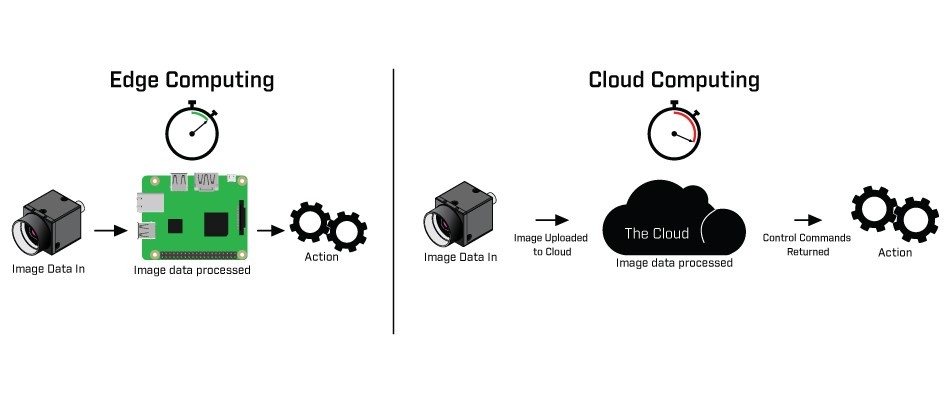
\includegraphics[width=0.9\textwidth]{figuren/iisedgecomputing.jpg}
	\caption{Edge vs. Cloud computing}
	\cite{flir-edge-computing}
	\label{fig:edge-vs-cloud}
\end{figure}

Er is gelukkig een grote 'paradigm shift' aan de gang waarbij men steeds meer machine learning gaat uitvoeren in embedded devices.
Dat is mogelijk omdat de embedded devices steeds sneller en beter worden in het verwerken van data.
Op die manier kunnen wij het machine learning model dichter bij de sensor plaatsen waardoor wij het benodigde netwerkverkeer minimaliseren.
Ook de latency of vertraging tussen opname en actie is veel kleiner. \cite{flir-edge-computing}

De ruwe data van de sensoren kan soms ook sensitieve informatie zoals gezichten of nummerplaten bevatten. Omdat we de data on-edge verwerken hoeven we die niet naar de cloud te sturen waar ze onderweg misschien onderschept kunnen worden. \cite{flir-edge-computing}
Het is echter niet zo simpel om de machine learning code, die geoptimaliseerd is voor multi-core servers, zomaar over te zetten naar de kleine, vaak single-core, microprocessors van deze embedded devices.
% In dit verslag leg ik het proces om een machine learning model getrained in python, over te zetten naar C code voor een microcontroller.

\subsection{Doel van het project}

Het doel van dit project is met een Convolutional Neural Netwerk (CNN) geluidsevents te classificeren.
Die geluidsevents kunnen bijvoorbeeld spraak, een handenklap, gefluit of achtergrondgeluid zijn.
Dat is relatief simpel uit te voeren op een normale PC, maar het is dus niet praktisch om alle geluidsdata van meerdere meetpunten centraal te verwerken in real time.
Ook is het niet kost-effectief om overal aparte PC's te plaatsen. In dit project ga ik dus het getrained CNN op een microcontroller uitvoeren om geluid van de ingebouwde microfoon te classificeren.

\section{Log-Mel feature extraction}

Het is mogelijk om een CNN te trainen op de onverwerkte geluidsdata.
Er zijn echter veel grotere modellen voor nodig, tot 34 lagen diep, en zal daarom ook sneller vatbaar voor overfitting. \cite{IEEE:very-deep-cnn-raw-waveforms}
Daarom is er toch een feature extraction stap gemaakt om de onverwerkte geluidsdata om te rekenen naar een Log-Mel spectrogram.
Dit Log-Mel spectrogram is eigenlijk een gewoon spectrogram waarvan we de frequentiebanden een beetje vervormd hebben zodat ze beter overeenkomen met de menselijke perceptie van geluid. \cite{enwiki:mel-freq-cepstrum}

\begin{no-awa} % Zorgt ervoor dat de latex-2-awa parser deze environment negeert
De  Log-Mel feature extraction gebeurt in deze 5 stappen:

\begin{enumerate}
	\item DC-Normalisation
	      \begin{itemize}
		      \item Hiervoor gebruiken we een eerste orde IIR filter:
		            \begin{itemize}[label={}]
			            \item \(y\left[ n \right] = x\left[ n \right] - x\left[ n - 1 \right] -0.999 \cdot y\left[ n - 1 \right]\)
		            \end{itemize}
	      \end{itemize}

	\item Framing and windowing
	      \begin{itemize}
		      \item Eerst deel ik de audio op in frames van 32 ms die elk 10 ms overlappen met elkaar
		      \item Daarna pas ik een Hamming-venster toe om hoogfrequente ruis te vermeiden \cite{enwiki:windowing}
	      \end{itemize}

	\item Discrete Fourier Transform (DFT)
	      \begin{itemize}
		      \item Met de DFT transformeren we elke frame van het tijdsdomein naar het frequentiedomein
		      \item We padden de frames totdat ze een macht van 2 zijn. Zo kunnen we het Fast Fourier Transform (FFT) algoritme gebruiken. Dit is sneller en accurater dan de normale DFT als er omdat er bij de gewone DFT meer afrondingsfouten kunnen gebeuren. \cite{enwiki:FFT}
		      \item Het resultaat is een vector met de magnitudes van elke frequentie in het signaal. Die vector is zeer hoogdimensionaal en is niet optimaal voor geluidsherkenning.
	      \end{itemize}

	\item Mel-frequency warping
	      \begin{itemize}
		      \item Mel-frequency warping transformeert de originele hoogdimensionale frequentievector naar een mel-frequency vector. Zie Figuur~\ref{fig:mel-bands}.
		            \begin{itemize}[label={}]
			            \item \(f_{mel} = 2595\log_{10}(1 + \frac{f}{700})\)
		            \end{itemize}
		      \item Die mel-frequency vector bevat minder frequentiebanden en is daardoor veel lager in dimensies. De mel-banden zijn echter zo verspreid zodat ze veel beter overeenkomen met de menselijke perceptie van geluid.
	      \end{itemize}

	\item Feature normalisation and scaling
	      \begin{itemize}
		      \item Tenslotte normaliseren we de logaritmes van de mel-magnitudes zodat het gemiddelde nul is, en de standaardafwijking één is:
		            \begin{itemize}[label={}]
			            \item \(m'_b = \frac{\ln\left( m_b \right) - \mu_b}{\sigma_b}\)
		            \end{itemize}
		      \item Als allerlaatste pre-processingstap gaan we de data schalen zodat die zich in het interval \(\left[ -1,1 \right]\) bevind. Zo kunnen ze opgeslagen worden in Q0.7 formaat. (Zie hoofdstuk \ref{section:Qm.f} op pagina \pageref{section:Qm.f})
	      \end{itemize}
\end{enumerate}
\end{no-awa}


\begin{figure}[ht]
	\centering
	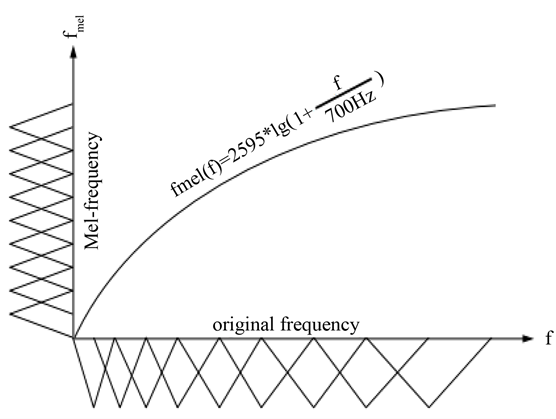
\includegraphics[width=0.7\textwidth]{figuren/mel-frequency.png}
	\caption{Mel-frequency warping}
	\cite{efficient-feature-extraction}
	\label{fig:mel-bands}
\end{figure}


\section{Convolutional Neural Network (CNN)}

\subsection{Structuur van ons CNN-model}

\subsection{Training}
\subsubsection{Resultaten}


\section{Edge implementatie}

\subsection{Kwantisatie van ons CNN-model}
\subsubsection{Qm.f formaat}
\label{section:Qm.f}

\subsection{Experiment met microfoon}
\subsubsection{Resultaten}


\section{Conclusie}